 \documentclass[a4paper]{article}

%% Language and font encodings
\usepackage[spanish]{babel}
\usepackage{fontspec}

%% Sets page size and margins
\usepackage[a4paper,top=3cm,bottom=2cm,left=3cm,right=3cm,marginparwidth=1.75cm]{geometry}

%% Useful packages
\usepackage{amsmath,amsthm,amssymb,amsfonts}
\usepackage{graphicx}
\usepackage[colorinlistoftodos]{todonotes}
\usepackage[colorlinks=true, allcolors=blue]{hyperref}
\usepackage{braket}
\usepackage{enumitem}


\newcommand{\R}{\mathbb{R}}
\newcommand{\N}{\mathbb{N}}
\newcommand{\Z}{\mathbb{Z}}
\providecommand{\C}{\mathbb{C}}

\theoremstyle{definition}
\newtheorem{defin}{Definición}

\theoremstyle{plain}
\newtheorem{theorem}[defin]{Teorema}
\newtheorem{corollary}[defin]{Corolario}



\title{Taller 3\\ Física Computacional I}

\author{Daniela Andrea Torres Gómez\\ C.C 1.036.665.120

}

\date{}

\begin{document}
\maketitle

%\begin{abstract}
%Your abstract.
%\end{abstract}


\section*{Oscilador Armónico}



Una masa $m$ es suspendida de un resorte de constante $k$. La masa se desplaza del equilibrio por una distancia $y_0$ y se suelta. El movimiento resultante se describe por la ecuación \ref{ec_1}, es decir, es un oscilador armónico con una frecuencia angular de oscilación dada por $\omega = \sqrt{\frac{k}{m}}$. 

\begin{equation}
 \ddot{y} + \omega^2 y = 0
 \label{ec_1}
\end{equation}

Esta ecuación diferencial de segundo orden se puede convertir en un sistema de 2 ecuaciones diferenciales acopladas de primer orden:

\begin{align*}
 \dot y = p_y & \\
 \dot p_y = -\omega^2 y
\end{align*}

\rule{145 mm}{0.1 mm}



\subsection{Resultados}



\begin{figure}[H]
\begin {center}
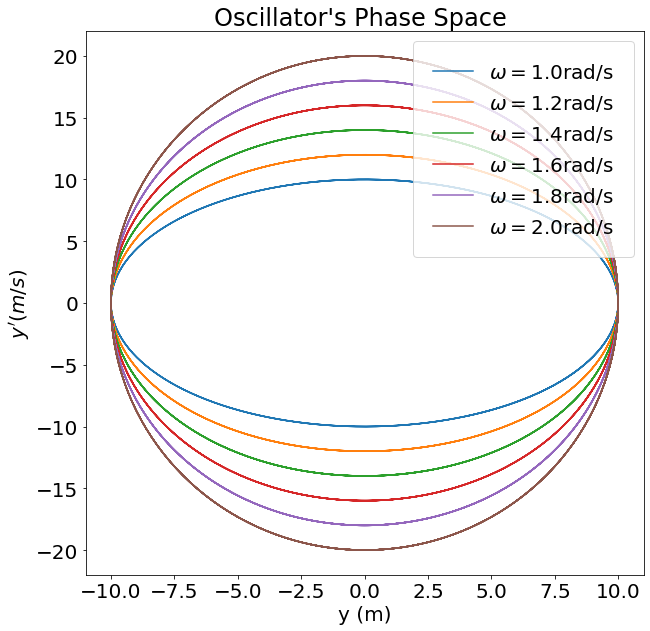
\includegraphics[width=0.5\textwidth]{output_2_3.png}
\caption{Espacio de fase del Oscilador Armónico}
\label{fig:PhaseH}
\end {center}
\end{figure}


\begin{figure}[H]
\begin {center}
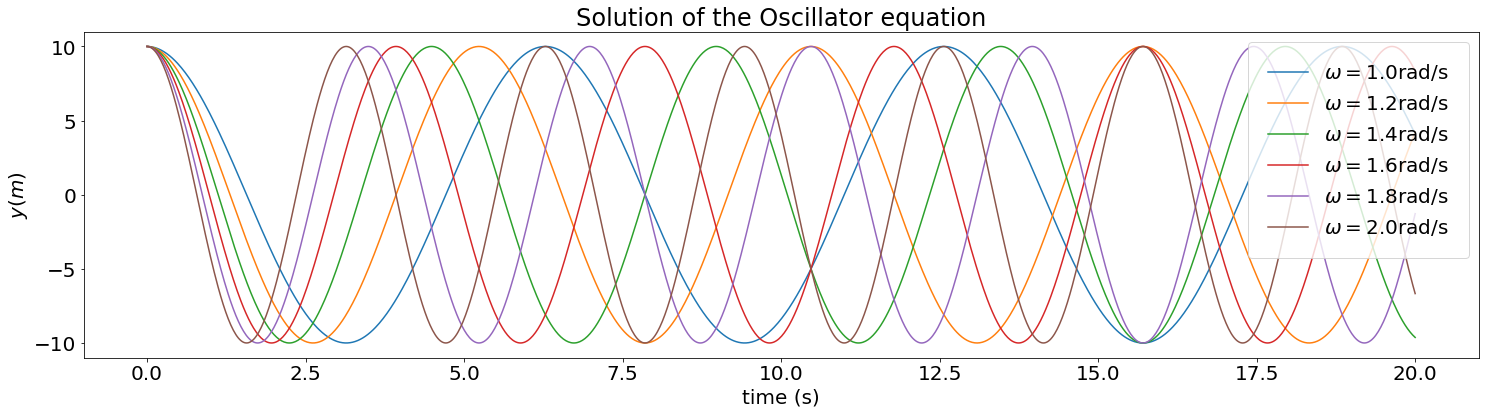
\includegraphics[width=0.9\textwidth]{output_2_2.png}
\caption{Solución al Oscilador Armónico}
\label{fig:solutionH}
\end {center}
\end{figure}


Dadas las condiciones iniciales $y(0) = y_0 = 10m $ y $p_y(0) = 0$, el movimiento del oscilador en el tiempo esta dado por la figura \ref{fig:solutionH}:


Se puede observar que el resultado es una función coseno, tal como se esperaba. Lo único que se modifica a medida que aumenta la frecuencia, es el periodo de oscilación, puesto que la amplitud de la onda solo está dada por las condiciones iniciales. 

Se encuentra que el único punto fijo que satisface el sistema es $P =(0, 0)$. Para hallar su estabilidad, se encuentra la matriz asociada al sistema de ecuaciones y se encuentra la traza y determinante de esta. Según la teoría de sistemas dinámicos, en el diagrama de bifurcación traza - determinante, el punto de equilibrio encontrado es un centro, y por lo tanto, es un punto estable. Los resultados se pueden ver en el la figura \ref{fig:PhaseH} correspondiente al espacio de fase. Al incrementar la frecuencia de oscilación, el elipsoide aumenta su dimensión en dirección del momentum ($y'$), pero se mantiene de igual tamaño en el eje de la posición ($y$). 



\section*{Oscilador Amortiguado}

Ahora, con los mismos parámetros y condiciones iniciales del oscilador armónico pero con un amortiguamiento $\gamma$. El movimiento está dado por la ecuación diferencial de segundo orden \ref{ec_2}.

\begin{equation}
 \ddot y + 2\gamma \omega_o \dot y + \omega_o^2  y = 0
 \label{ec_2}
\end{equation}

Esta ecuación diferencial de segundo orden se puede convertir en un sistema de 2 ecuaciones diferenciales acopladas de primer orden:

\begin{align*}
 \dot y  = p_y & \\
 \dot p_y = - 2\gamma \omega_o p_y - \omega_o^2  y 
\end{align*}

Igualmente, se encuentra que el punto fijo es $P =(0, 0)$ y por la teoría de sistemas dinámicos, la matriz de coeficientes queda como:

\begin{align*}
    \begin{pmatrix}
        0 & 1\\
        -\omega^2 & -2\gamma
    \end{pmatrix}
\end{align*}

Por lo cual el discriminante es $\gamma^2 - \omega^2 $. Como se asume el caso subamortiguado, debe cumplirse que el discriminante es menor a cero y por lo tanto en el espacio de fase se ven espirales. Además, como el negativo  de la traza es $Tra=2\gamma$ y $\gamma > 0$, en el diagrama traza - determinante se encuentra que el punto fijo es asintóticamente estable, es decir, que a medida que pasa el tiempo, el oscilador tenderá al punto $(y, py) = (0,0)$. 

\begin{equation*}
    
\end{equation*}

\rule{145 mm}{0.1 mm}

\subsection{Resultados}

\begin{figure}[H]
\begin {center}
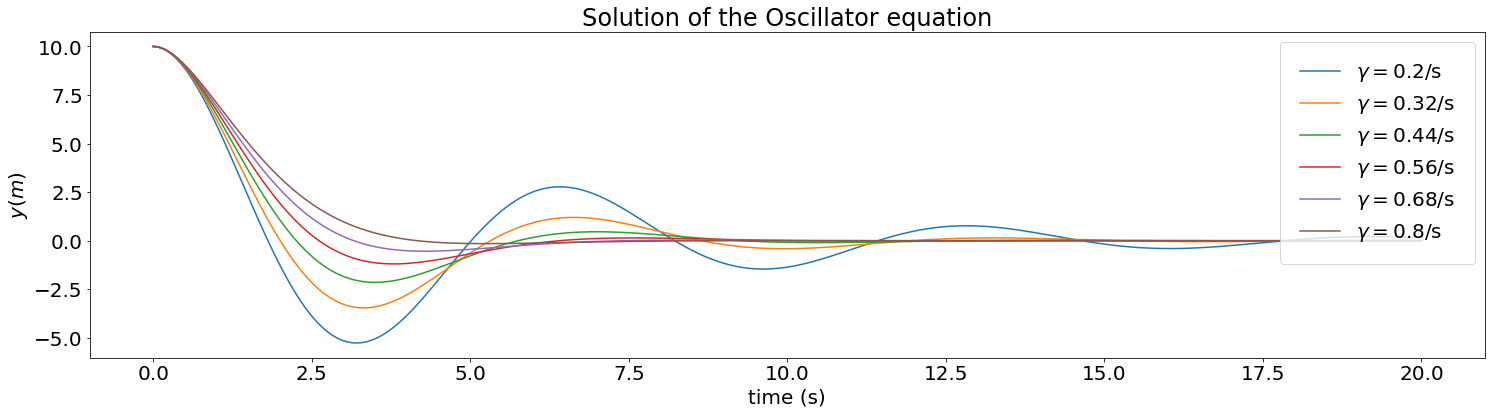
\includegraphics[width=0.9\textwidth]{output_2_0.png}
\caption{Solución al Oscilador Amortiguado}
\label{fig:solutionA}
\end {center}
\end{figure}


\begin{figure}[H]
\begin {center}
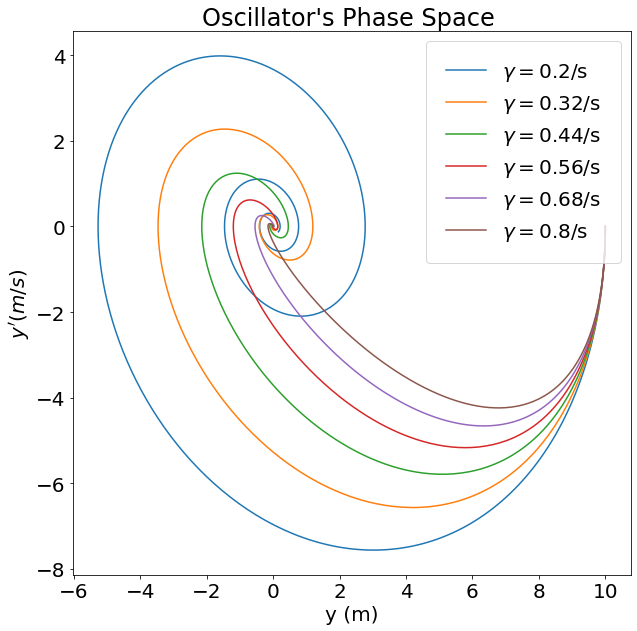
\includegraphics[width=0.5\textwidth]{output_2_1.png}
\caption{Espacio de fase del Oscilador Amortiguado}
\label{fig:PhaseA}
\end {center}
\end{figure}

Se ve que a medida que aumenta el coeficiente de amortiguamiento (para el caso subamortiguado), el resorte tiende más rápido al punto de equilibrio como se ve en el diagrama de\ref{fig:PhaseA}, y por lo tanto, la amplitud del movimiento tambíen se hace menor mucho más rápido como se ve en la figura \ref{fig:solutionA}.


\end{document}